\documentclass[article,colorback,accentcolor=tud4c, 11pt]{tudreport}
%\usepackage{ngerman}

\usepackage[stable]{footmisc}
\usepackage[ngerman]{hyperref}

\usepackage{longtable}
\usepackage{multirow}
\usepackage{booktabs}
\usepackage[utf8]{inputenc}
\usepackage[export]{adjustbox}
\graphicspath{ {screens/} }

\hypersetup{%
  pdftitle={TUD Corporate-Design f"ur {\LaTeX}},
  pdfauthor={C. v. Loewenich und J. Werner},
  pdfsubject={Beispieltext},
  pdfview=FitH,
  pdfstartview=FitV
}

\setcounter{seclinedepth}{1}

%%% Zum Tester der Marginalien %%%
  \newif\ifTUDmargin\TUDmarginfalse
  %%% Wird der Folgende Zeile einkommentiert,
  %%% werden Marginalien gesetzt.
  % \TUDmargintrue
  \ifTUDmargin\makeatletter
    \TUD@setmarginpar{2}
  \makeatother\fi
%%% ENDE: Zum Tester der Marginalien %%%

\newlength{\longtablewidth}
\setlength{\longtablewidth}{0.7\linewidth}
\addtolength{\longtablewidth}{-\marginparsep}
\addtolength{\longtablewidth}{-\marginparwidth}


% \settitlepicture{tudreport-pic}
% \printpicturesize

\title{Internet Praktikum of Telecooperation Group - Winter Term 2018/2019\\
	Project Topic: Interactive Door Panel for Office Availability\\ Team Foxtrot}
\subtitle{Artem Vopilov (email: mister.0026@yandex.ru)\\Florian Schunk (email: florian.schunk@stud.tu-darmstadt.de)\\ Javier Ochoa Serna (email: jochoaserna@hotmail.com)\\
	Pramod Pramod (email: pramod.pramod@stud.tu-darmstadt.de) \\ Frank Langoulant (email: fl1001@rbg.informatik.tu-darmstadt.de)}
%\setinstitutionlogo[width]{TUD_sublogo}
\uppertitleback{(\textaccent{\textbackslash uppertitleback})}
\lowertitleback{(\textaccent{\textbackslash lowertitleback})\hfill\today}
\institution{Telecooperation Group\\
	S2|02 A114
	Hochschulstraße 10
	64289 Darmstadt}
%\dedication{Hier ist gen"ugend Platz\\
%  f"ur eine Widmung (\textaccent{\textbackslash dedication}).\\
%  \strut\\
%  F"ur Annelore Schmidt\\
%  aus dem Referat Kommunikation.\\
%  Sie hat immer ein offenes Ohr\\
%  f"ur unsere Fragen und Anregungen.}


\begin{document}
	\maketitle
	\begin{abstract}
		In this project we implement a door panel application designed to run on  Android Tablet as well as the counterpart application designed to run on android smartphones. The intention is to display information about the office room the doorpanel is assigned to as well as the workers in this office and their availability status. If the workers don't want to be disturbed by visitors cumming by, the application provides the means to request an appointment as well as to send a message to a worker.
	\end{abstract}  
	
	\tableofcontents
	%%\part{Lorem Ipsum (\textbackslash part)\label{part_lorem}}
	\newpage
	
	\section{Motivation}
	
Traditional door panel signs printed on paper may be quite common but they lack a lot of possibilities. Every time there is a change concerning the workers assigned to the office room, the sign needs to be reprinted and replaced. Even more important, the workers have no means to indicate to visitors passing by and maybe wanting to talk to a worker inside the office if they are welcome to enter or if a disturbance is currently inappropriate. \\

In order to change that we implemented an interactive door panel application to meet the requirements of up to date offices and their personnel. It consists of an application intended to run on an Android smartphone and an application ro run on the Android smartphones of the workers. \\

The tablet application displays the workers who are currently assigned to the office room and provides the possibility to send a message to the worker as well as to request an appointment within timeslots the workers can choose separately. \\

The smartphone application provides the possibility to the worker to change his availability status, to receive and answer messages, to access his calendar and to change the personal information about himself/herself such as picture, phone number and email adress.It also allows the worker to choose a Google calendar that is connected to the application and were confirmed appointments are stored. Finally it also allows the worker to choose timeslots that are available for appointment request to visitors.\\

This door panel application is intended to support workers in an office room to handle messages and appointment request of visitors without being disturbed or interrupted during their work.

 
\section{Structure}

For easier understanding, we will call the android application designed to run on a tablet placed outside of the workers office 'doorpanel app' und the counter part application designed to run on workers android smartphone 'mobile app'.\\
\subsection{Structural Overview}
This application is designed as a server client architecture. All informations are stored using MongoDB, the communication is handled by a NodeJS Server and messages are distributed using Firebase. Google calendar is adressed by the doorpanel app and mobile app directly. Figure 1 shows an overview over the architecture.

	 \begin{figure}
	   %\centering
	   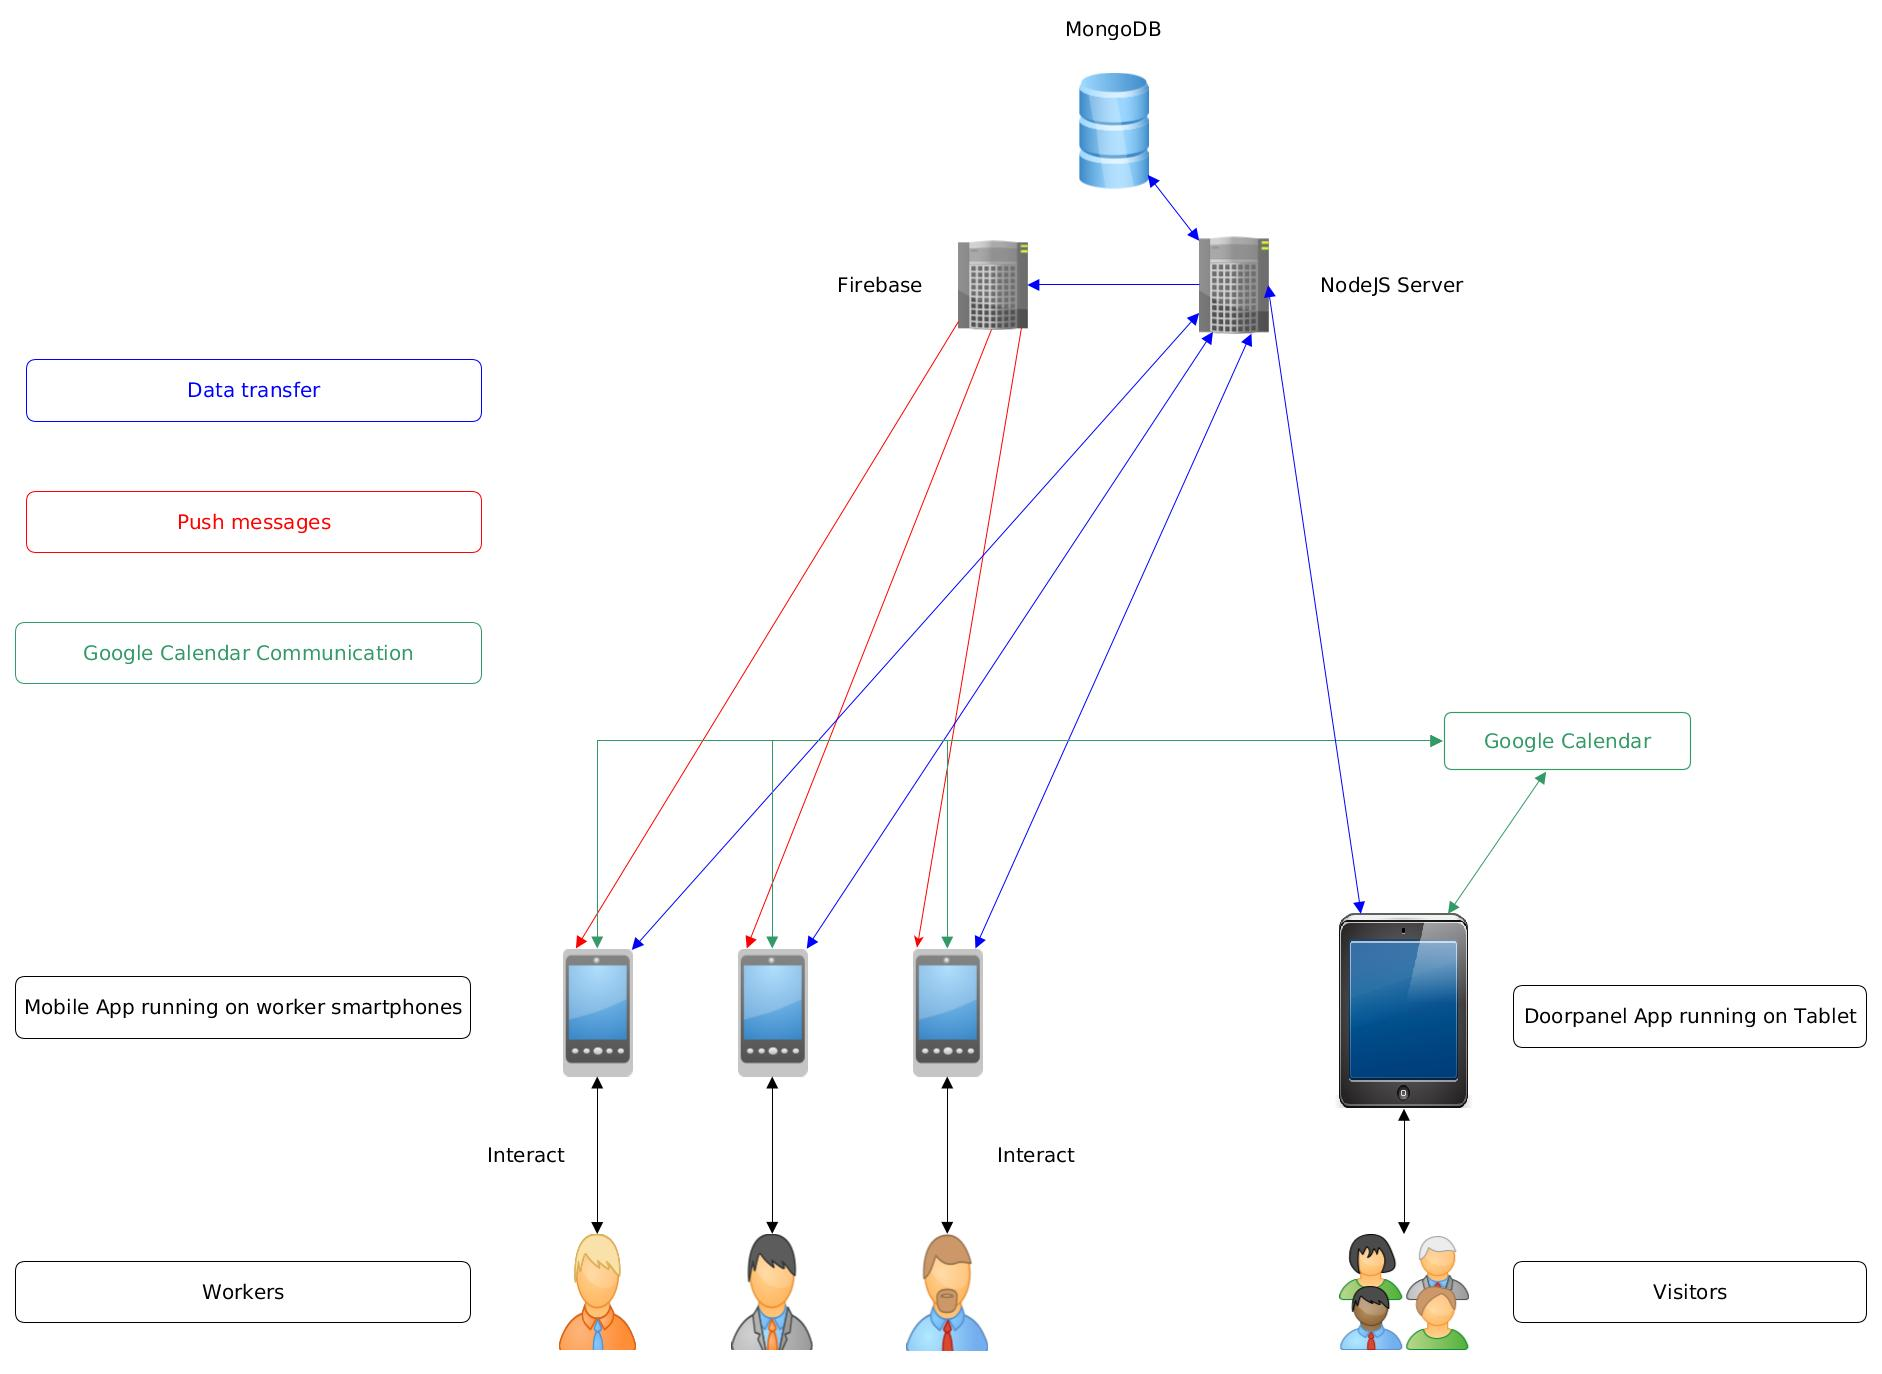
\includegraphics[max size={\textwidth}{\textheight}]{overview}
	    \caption[Structural overview]{Basic communication}
	 \end{figure}
	
	
	
	
\subsection{Description of elements and their interaction}
To be able to store any information the application needs access to a MongoDB database. The location is stored in $server/config/default.json$

To enable communication between the elements all elements the NodeJS server needs to be reachable. The IP-Adress of the hosting machine is stored in $'RetrofitClient.java'$ as string called $'BASE_URL'$. The file $'RetrofitClient.java'$ is located at $'src/main/java/.../network/RetrofitClient.java'$ in both application parts.
	
	
\subsection{Google authentication}
Because we use Google APIs for accessing the Google Calendar, we need to follow the Google authentication procedure.
Google requires that developers provide the key that is used for compiling in the Google Developer Console.
To do so, visit the following website:\\ \\
$https://console.developers.google.com/apis/credentials?folder\\=\&organizationId=\&project=winter-time-228212$\\ \\
Login with email $'doorpaneltest@gmail.com'$ and password $'FoxtroTT$'
There click on $'Create Credentials'$ and then on $'OAuth Client ID'$ Next select $'Android'$.
Then you are asked to select a name, here you could use anything, but please be so kind and state your real name here, so it is easier for us to manage.
Also you need to provide your key. Google tells you to run\\ \\
\textit{keytool -exportcert -keystore path-to-debug-or-production-keystore -list -v} \\ \\
the path to the keystor should usually be\\ \\ $~/.android/debug.keystore$ \\ \\
however I got an error that I can't give 2 commands at the same time, so I removed the \\$-exportcert$
So my total command was the following:\\ \\
keytool -alias androiddebugkey -keystore ~/.android/debug.keystore -list -v\\ \\
More information is under:\\ \\
$https://support.google.com/cloud/answer/6158849?hl=en-GB\#\\installedapplications\&android$\\ \\
alternatively you can run the gradle task signingReport
Finally you have to choose\\ \\$de.tu\_darmstadt.foxtrot.foxtrot\_doorpanel\_app$\\ \\ as Package name	

\subsection{Dependencies \& Requirements}
This application is designed to work on Android version 9 (API Level 28)
The minimum Android version for this application to run is Android version 4.3 (API level 18). \\ \\
Packages needed for the NodeJS server to run:\\
\begin{itemize}
	\item Koa
	\item koa-router
	\item Koa-bodyparse
	\item mongoose
	\item firebase-admin
\end{itemize}

If the package 'NPM' is installed all those dependencies can easily by executing 'NPM install'.\\

	
\section{User Descripton}

	
\subsection{Basic Funtionality}
The doorpanel app running on a tablet displays the room number and the workers currently assigned to this office room. The app surface also displays a picture chosen by the worker, the position of the worker (eg 'Intern', 'Student', 'Professor') and the availability status also selected by the worker.
A visitor can select a worker to get further information about the worker (if entered) and also send this worker an instant message. For this a message text is needed as well as a name and an email adress.\\

Next to the worker a calendar symbol offers the visitor the possibility to send an appointment request. For this the visitor needs to choose an available timeslot determined by the worker and also enter a name, an email adress, an phone number and a message text.\\ \\

The mobile app is intended as a control and access unit for the worker. It provides the ability to access the linked Google calendar, to select the availability status with a predefined or individual text as well as to see and answer the messages send from visitors and any appointment requests.\\

The mobile app is also used to adapt personal settings such as changing the picture, changing phone number, email adress and room number, entering further personal information (eg current research or publications), define timeslots in which visitors can request appointments, selecting a calendar to link to the application and also to add new workers.
	
\subsection{Detailed explanation}

Figure 2 shows the main menu of the mobile app. It provides access to the calendar display, the selection of the availability status, the list of notifications and appointment requests as well as to the settings menu.\\

	\begin{figure}
	 \centering
	   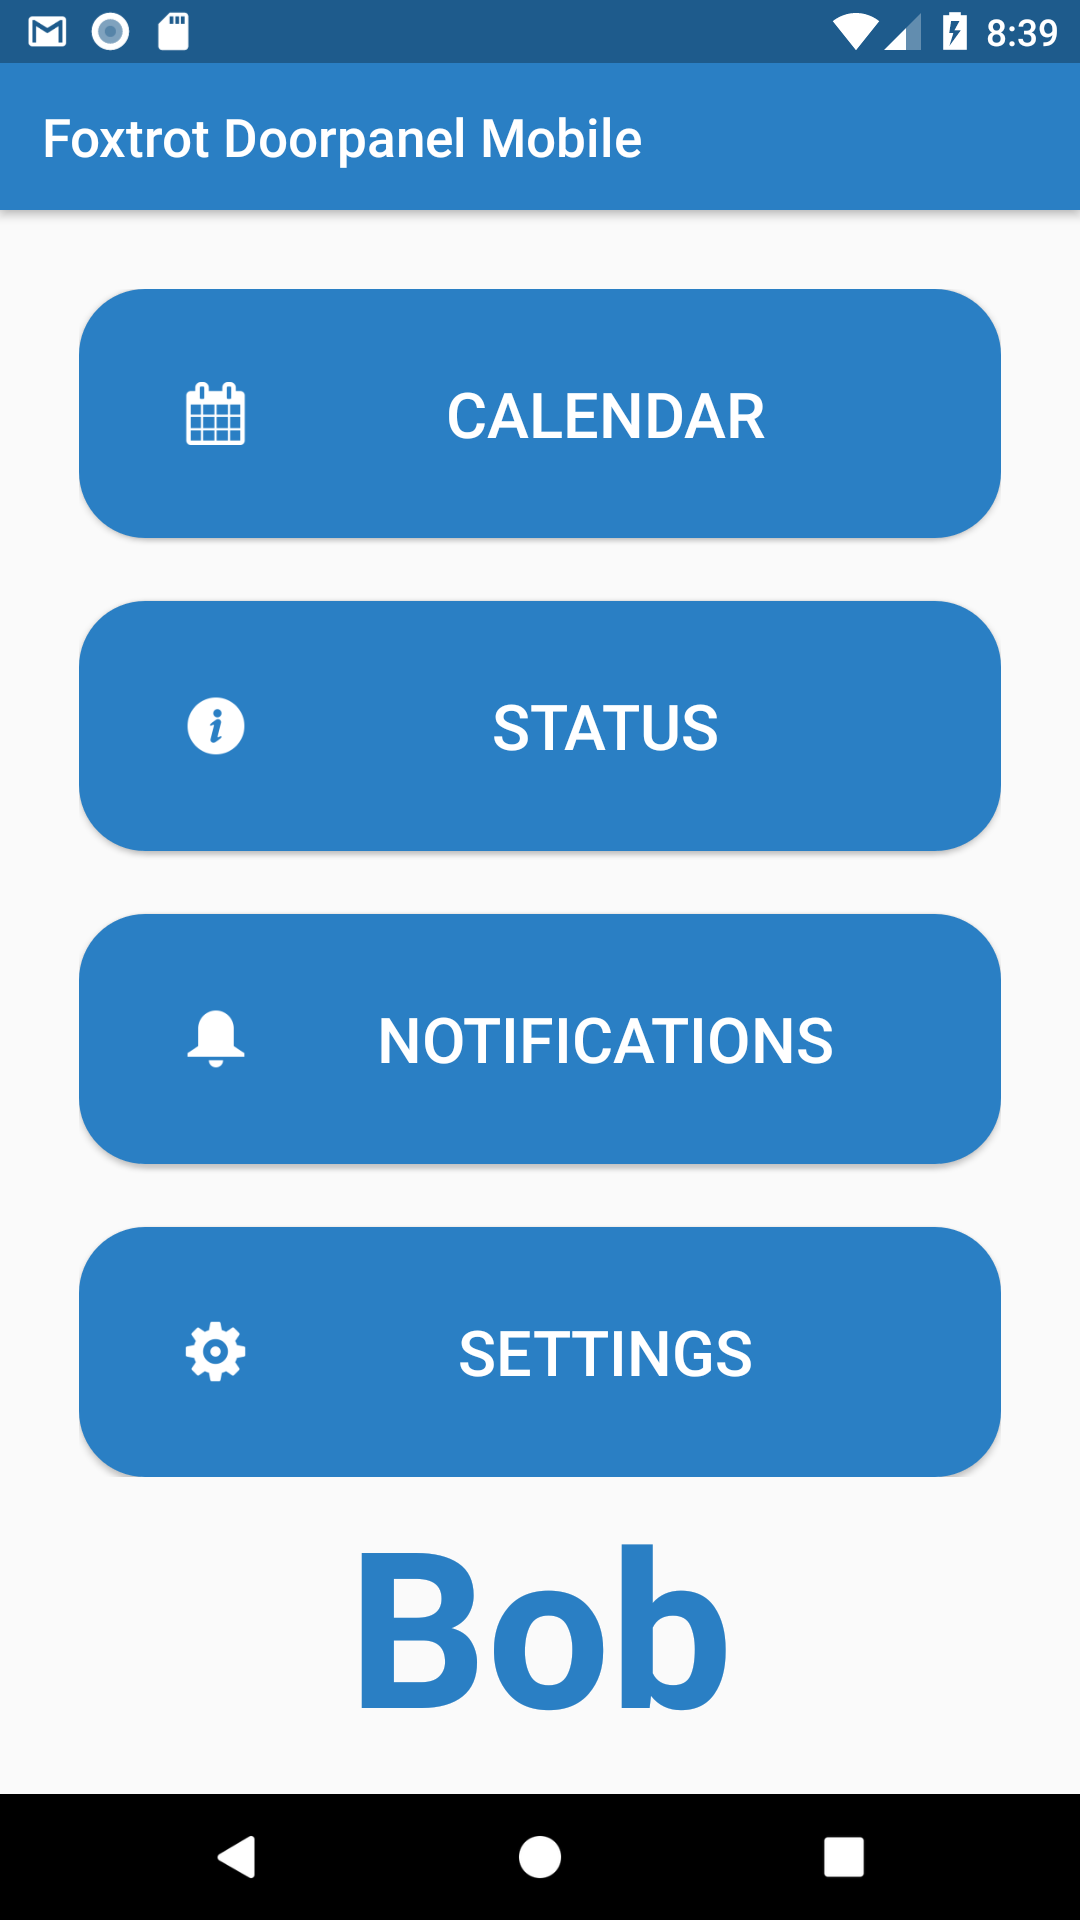
\includegraphics[width=30mm,scale=0.8]{mobile/Main-Screen.png}
	   \caption{Main Screen}
	\end{figure}

Figure 3 shows the menu to select a workers availability status. This menu is reached by the button 'status' on the main menu. The worker can choose between some predefined texts or enter an won description. The availability status is changed on the doorpanel app instantly.\\
 
	\begin{figure}
		\centering
		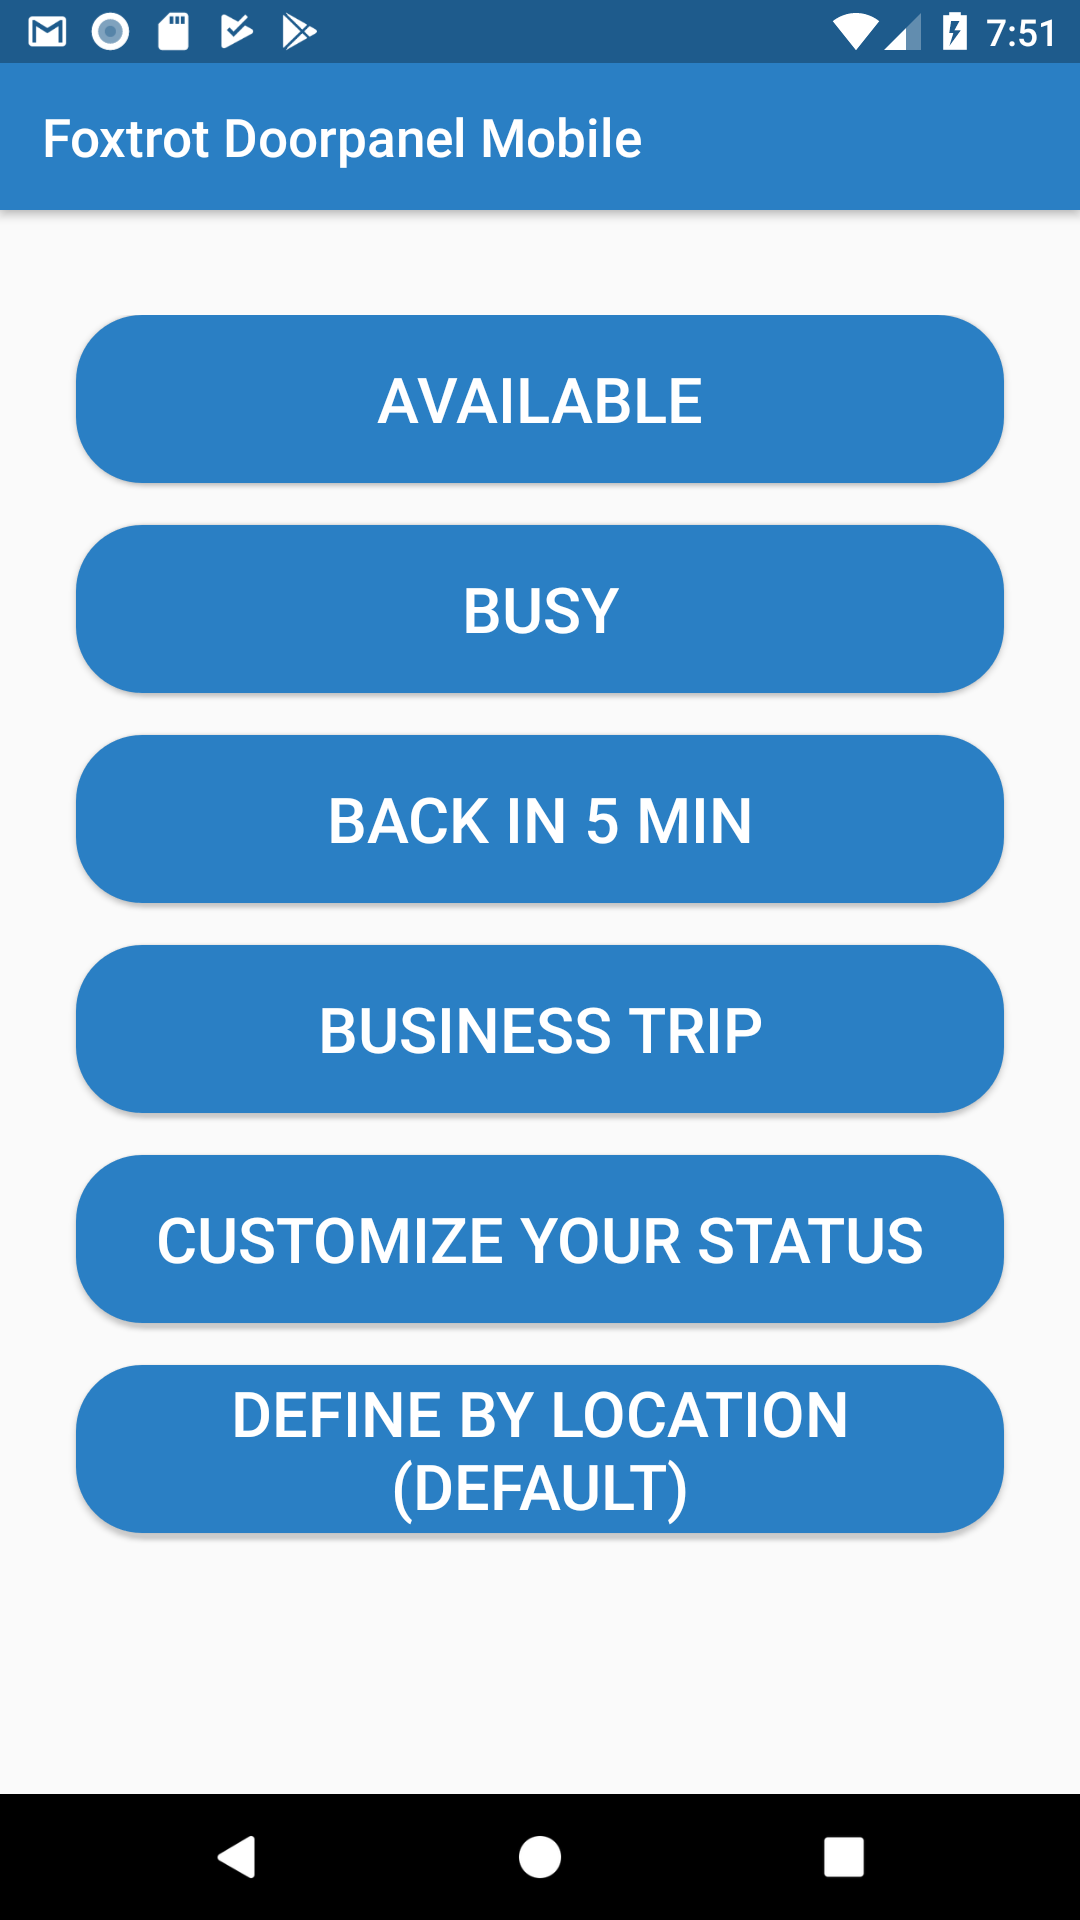
\includegraphics[width=30mm,scale=0.8]{mobile/Status-selection.png}
		\caption{Status Selection}
	\end{figure}
	
Figure 4 shows the list of notifications send from the doorpanel app to the mobile app. They are sorted chronologically. \\
 
	\begin{figure}
		\centering
		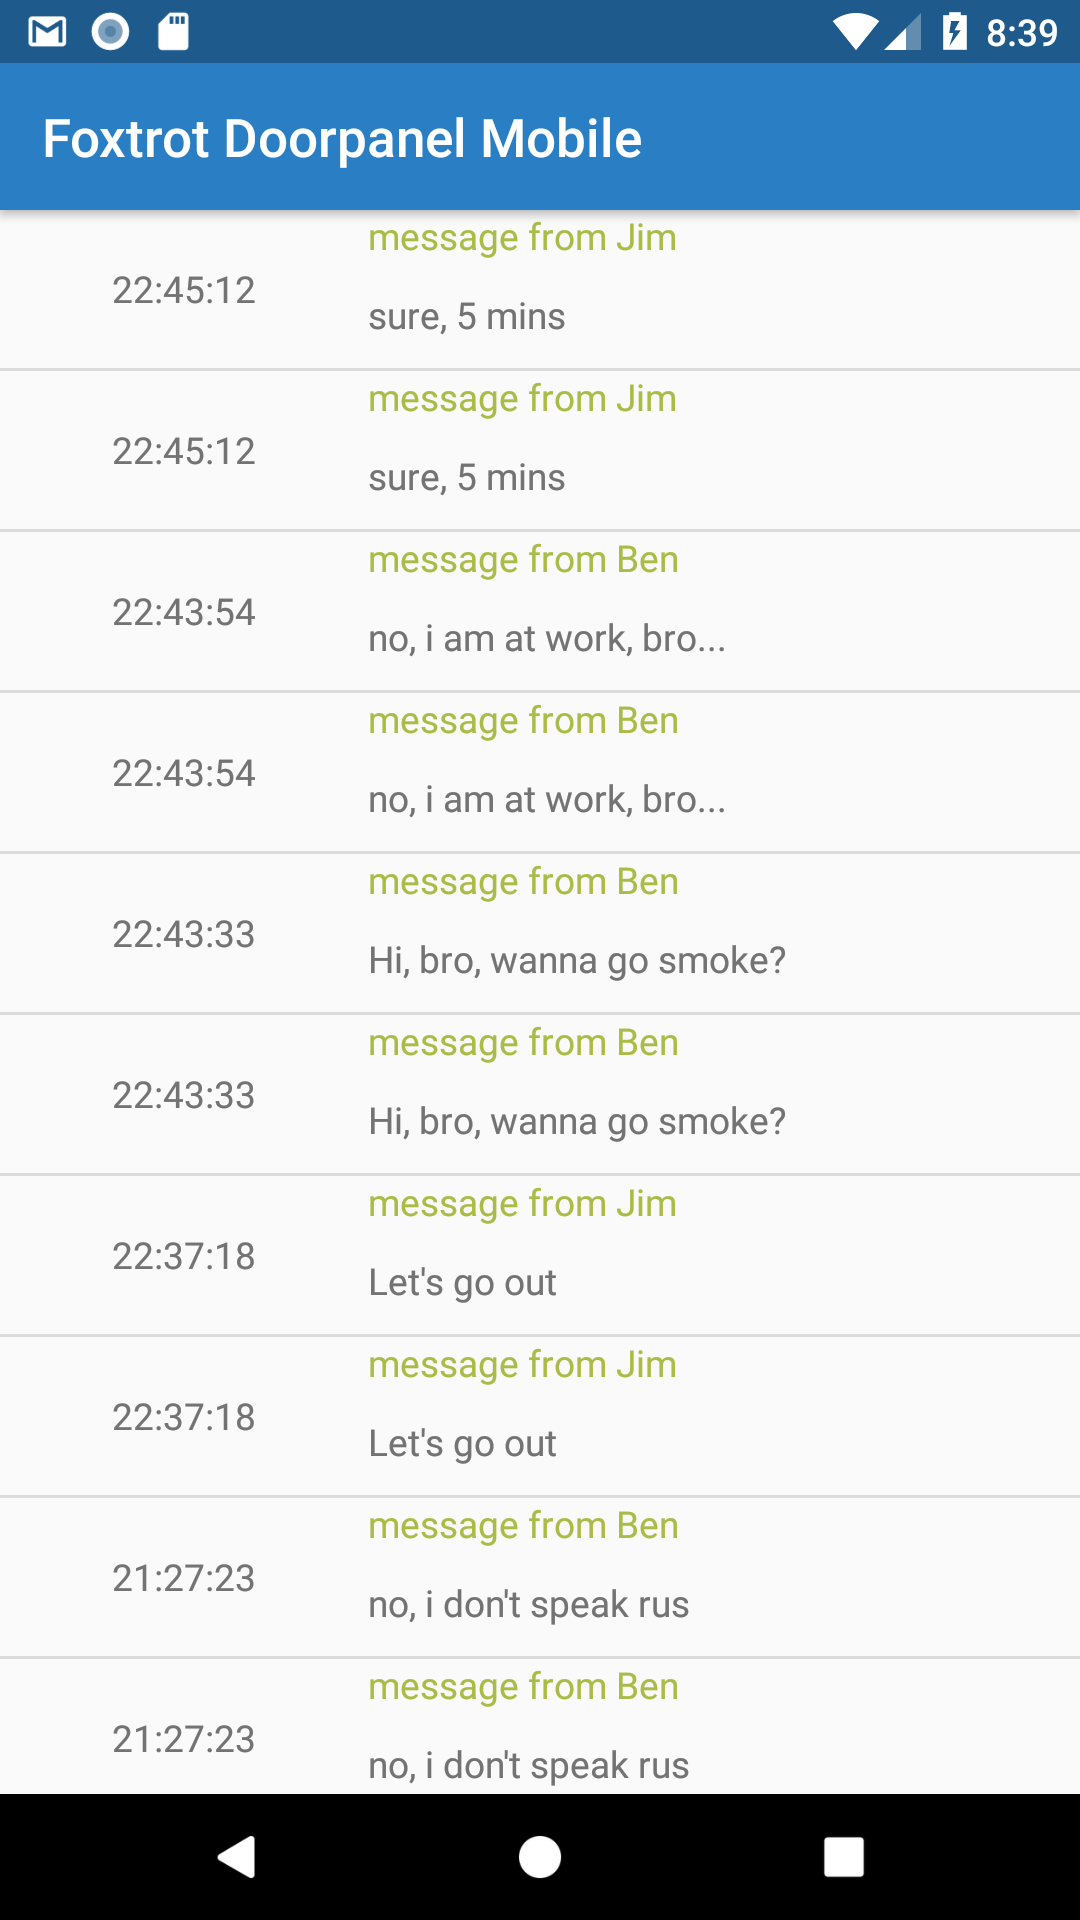
\includegraphics[width=30mm,scale=0.8]{mobile/Notifications.png}
		\caption{Notifications}
	\end{figure}

	\begin{figure}
		\centering
		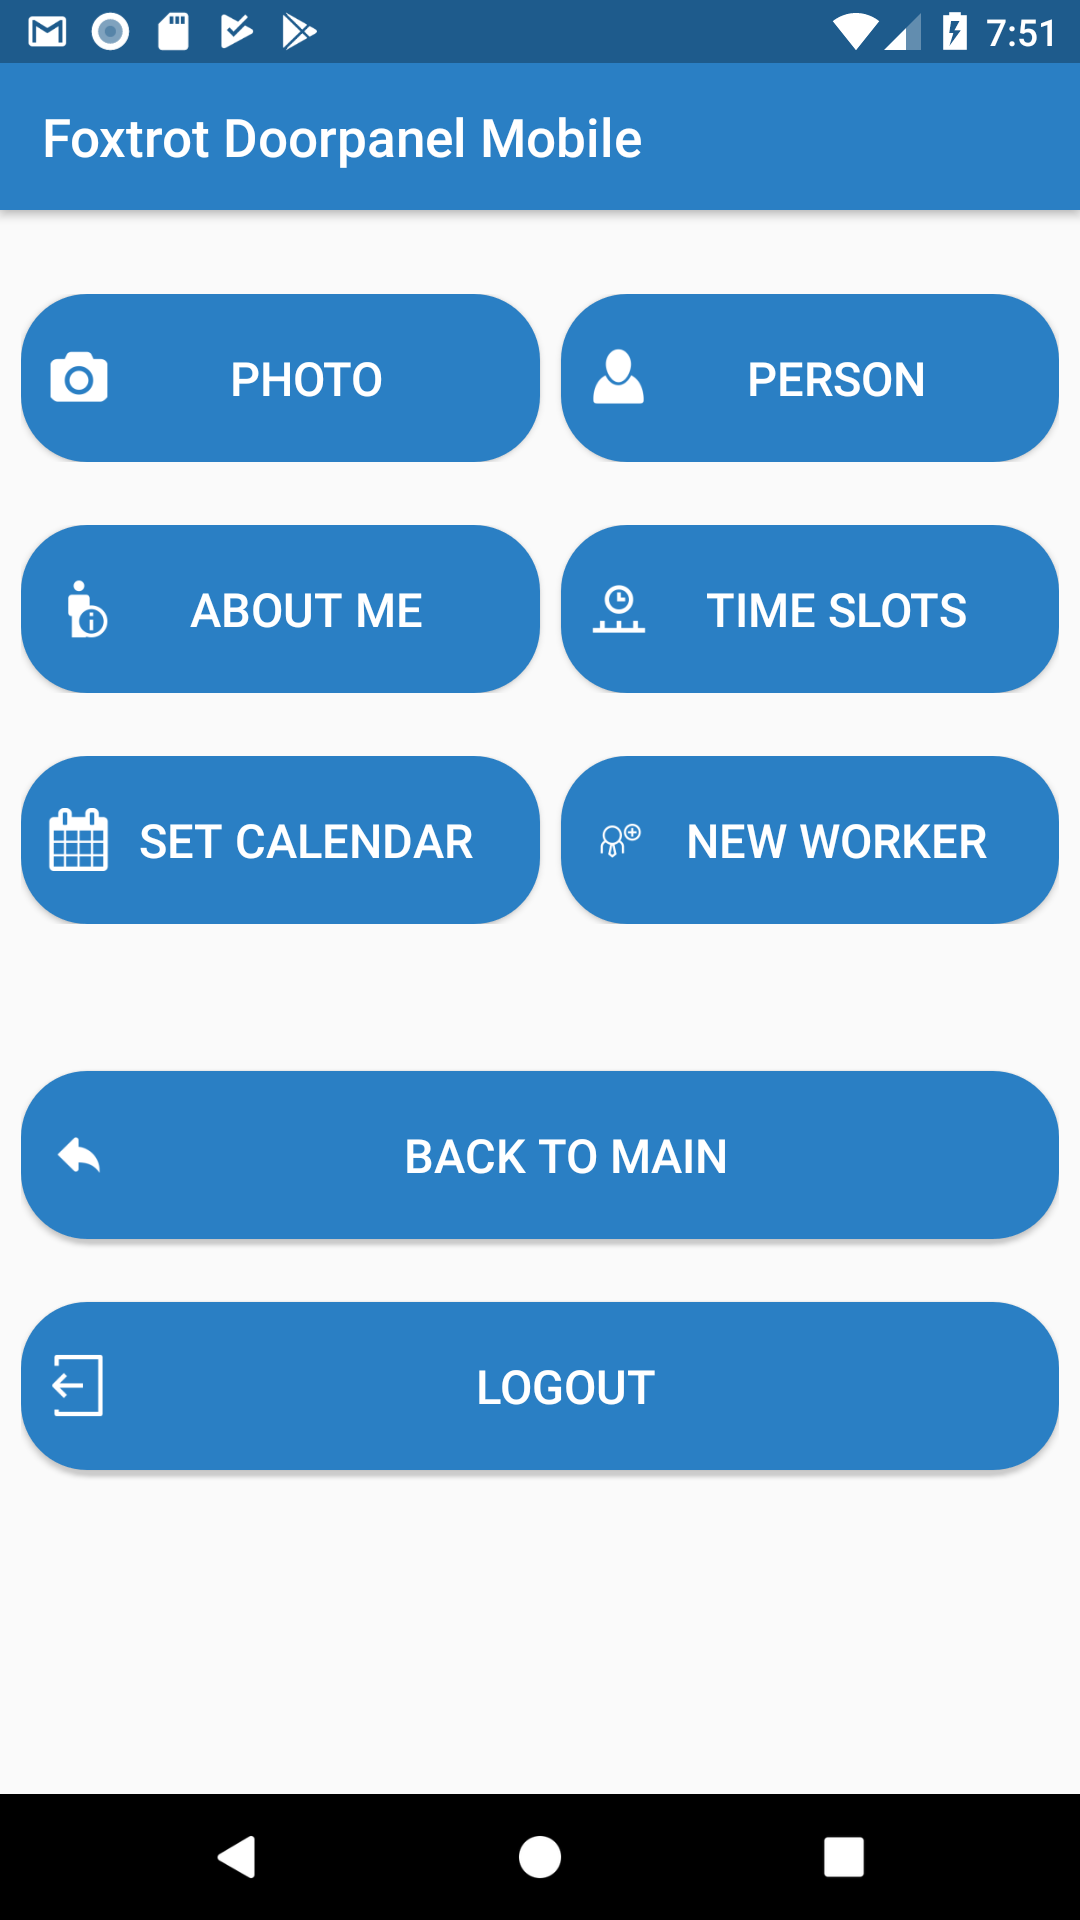
\includegraphics[width=30mm,scale=0.8]{mobile/Settings.png}
		\caption{Settings Main Level}
	\end{figure}	

Figure 5 shows the main settings menu. 

	%%\footnote{T.\ Pratchett: ''A guess? Well, that's good enough for physics!{``}}
	
	
	
	\listoffigures\addcontentsline{toc}{chapter}{\listfigurename}
\end{document}
